\documentclass[pdftex, 12pt, a4paper]{report}

\newcommand{\HRule}{\rule{\linewidth}{0.5mm}}
\usepackage{enumerate}
\usepackage{graphicx}
\bibliography{architecturaldesign.main.bib}
\usepackage[english]{babel}
\usepackage{fancyhdr}
\usepackage{pdfpages}

\begin{document}

\pagestyle{fancy}
\fancyhead{}
\fancyhead[LE, LO] {\today}
\fancyhead[CE, CO] {Architectural Design}
\fancyhead[RE, RO] {version 1}

\begin{titlepage}

\begin{center}


% Upper part of the page

\textsc{\Large Technische Universiteit Delft }\\[1.5cm]
\textsc{\large TI3800 Bachelorproject}\\[0.5cm]
\textsc{\normalsize A non-centralized approach to Video on Demand on mobile devices}\\[0.5cm]


% Title
\HRule \\[0.4cm]
{ \huge \bfseries Architectural Design}\\[0.4cm]

\HRule \\[1.5cm]

% Author and supervisor
\begin{minipage}{0.4\textwidth}
\begin{flushleft} \large
\emph{Authors:}\\
Martijn \textsc{Breet} \\ (1265458) \\ [0.1cm]
Jaap \textsc{van Touw} \\(1380753)\\ [0.1cm]
\end{flushleft}
\end{minipage}
\begin{minipage}{0.4\textwidth}
\begin{flushright} \large
\emph{Supervisor:} \\
Cor-Paul \textsc{Bezemer}
\end{flushright}
\end{minipage}
\vspace{30mm}
\begin{figure}[ht!]
\centering

\includegraphics[width=50mm]{TUDLogo.png}
\hspace{10mm}

\includegraphics[width=50mm]{pdslogo.png}
\label{overflow}
\end{figure}
\vfill

% Bottom of the page
{\large \today}

\end{center}

\end{titlepage}


\tableofcontents

\pagebreak

\chapter{Proposed Architecture}
In this chapter the proposed prototype will be separated into different subsystems to give more insight into how the team will build the system. First the different subsystems will be elucidated, followed by an explanation on how the different subsystems interact with each other. The way the system stores data is clarified in Section \ref{sec:perdata}. Different threads might try to alter the same part of data which causes a concurrency issue, when this would be possible and how the team will attempt to solve this is described in Section \ref{sec:conc}. How information flows from subsystem to subsystem in different use cases can be seen in Section \ref{sec:softctrl}. In the final section, we will explain how the system will deal with starting and stopping as well as crashes, how this will be implemented is explained in the final section.		%chapter + intro
\section{System composition}
In this section, the different subsystems are described, followed by how they are combined together to form the proposed architecture of the prototype.
\subsection{Subsystems}
\begin{itemize}
\item \textbf{VLC}
	\begin{itemize}
		\item LibVLCcore\\
This core manages the threads, loading/unloading modules (codecs, multiplexers, demultiplexers, etc.) and all low-level control in VLC.
		\item LibVLC\\
On top of libVLCcore, a singleton class libVLC acts as a wrapper class, that gives external applications access to all features of the core.
		\item VLC modules\\
VLC comes with more than 200 modules including various decoders and filters for video and audio playback. These modules are loaded at runtime depending on the necessity. The modules communicate with the hardware directly without using the previously described LibVLC wrapper class.
		\item Buffer Control\\
A buffer helps to ensure smooth playback, it puts media data from the storage in to the buffer to ready it for the VLC media player.
		\item VLC media player\\
The media player from VLC will be the Graphical User Interface(GUI) when the user is watching a video. The GUI will be explained more in depth in the GUI subsystem.
	\end{itemize}
\item \textbf{Tribler}
	\begin{itemize}
		\item Core\\
The core is the main part of Tribler and includes the control of all modules including LibTorrent.
		\item Libtorrent\\
Libtorrent is a C++ implementation of the BitTorrent protocol, which Tribler uses to download the different pieces of a requested file. For Video-on-Demand(VoD) it will do this according to the following download algorithm described by Petrocco et al\cite{libswift12}: The download algorithm discerns three priority tiers: high-, middle- and low-priority. The high priority section starts from the current playback position. First it downloads the pieces in this section in-order so that the user experiences continues playback. If no pieces can be downloaded from the high priority section, it will download the pieces in the mid priority section in a rarity first fashion to increase the availability of pieces in the swarm. If the middle priority pieces are also exhausted, it will download the low priority pieces in the same fashion. 
		\item Video Player Control\\
An important thing for Libtorrent is the current playback position because Libtorrent needs to get the right pieces for playback. The current playback position will be monitored by the Video Player Control.
	\end{itemize}
\item \textbf{GUI}
	\begin{itemize}
		\item Start\\
The GUI which is shown when the prototype is started, will show a start button. What happens when this button is pressed is further explained in the Section \ref{sec:comp}, which is about the composition of the different subsystems.
		\item VLC media player\\
The media player which comes with VLC for Android Beta has all the functionality needed for video playback control. It functions as the GUI when the user is watching a video. The user can use gesture controls to seek in the video, pause and then resume it and adjust the volume.
	\end{itemize}
\end{itemize}
\subsection{Composition}
\label{sec:comp}
\begin{figure}[h!]
	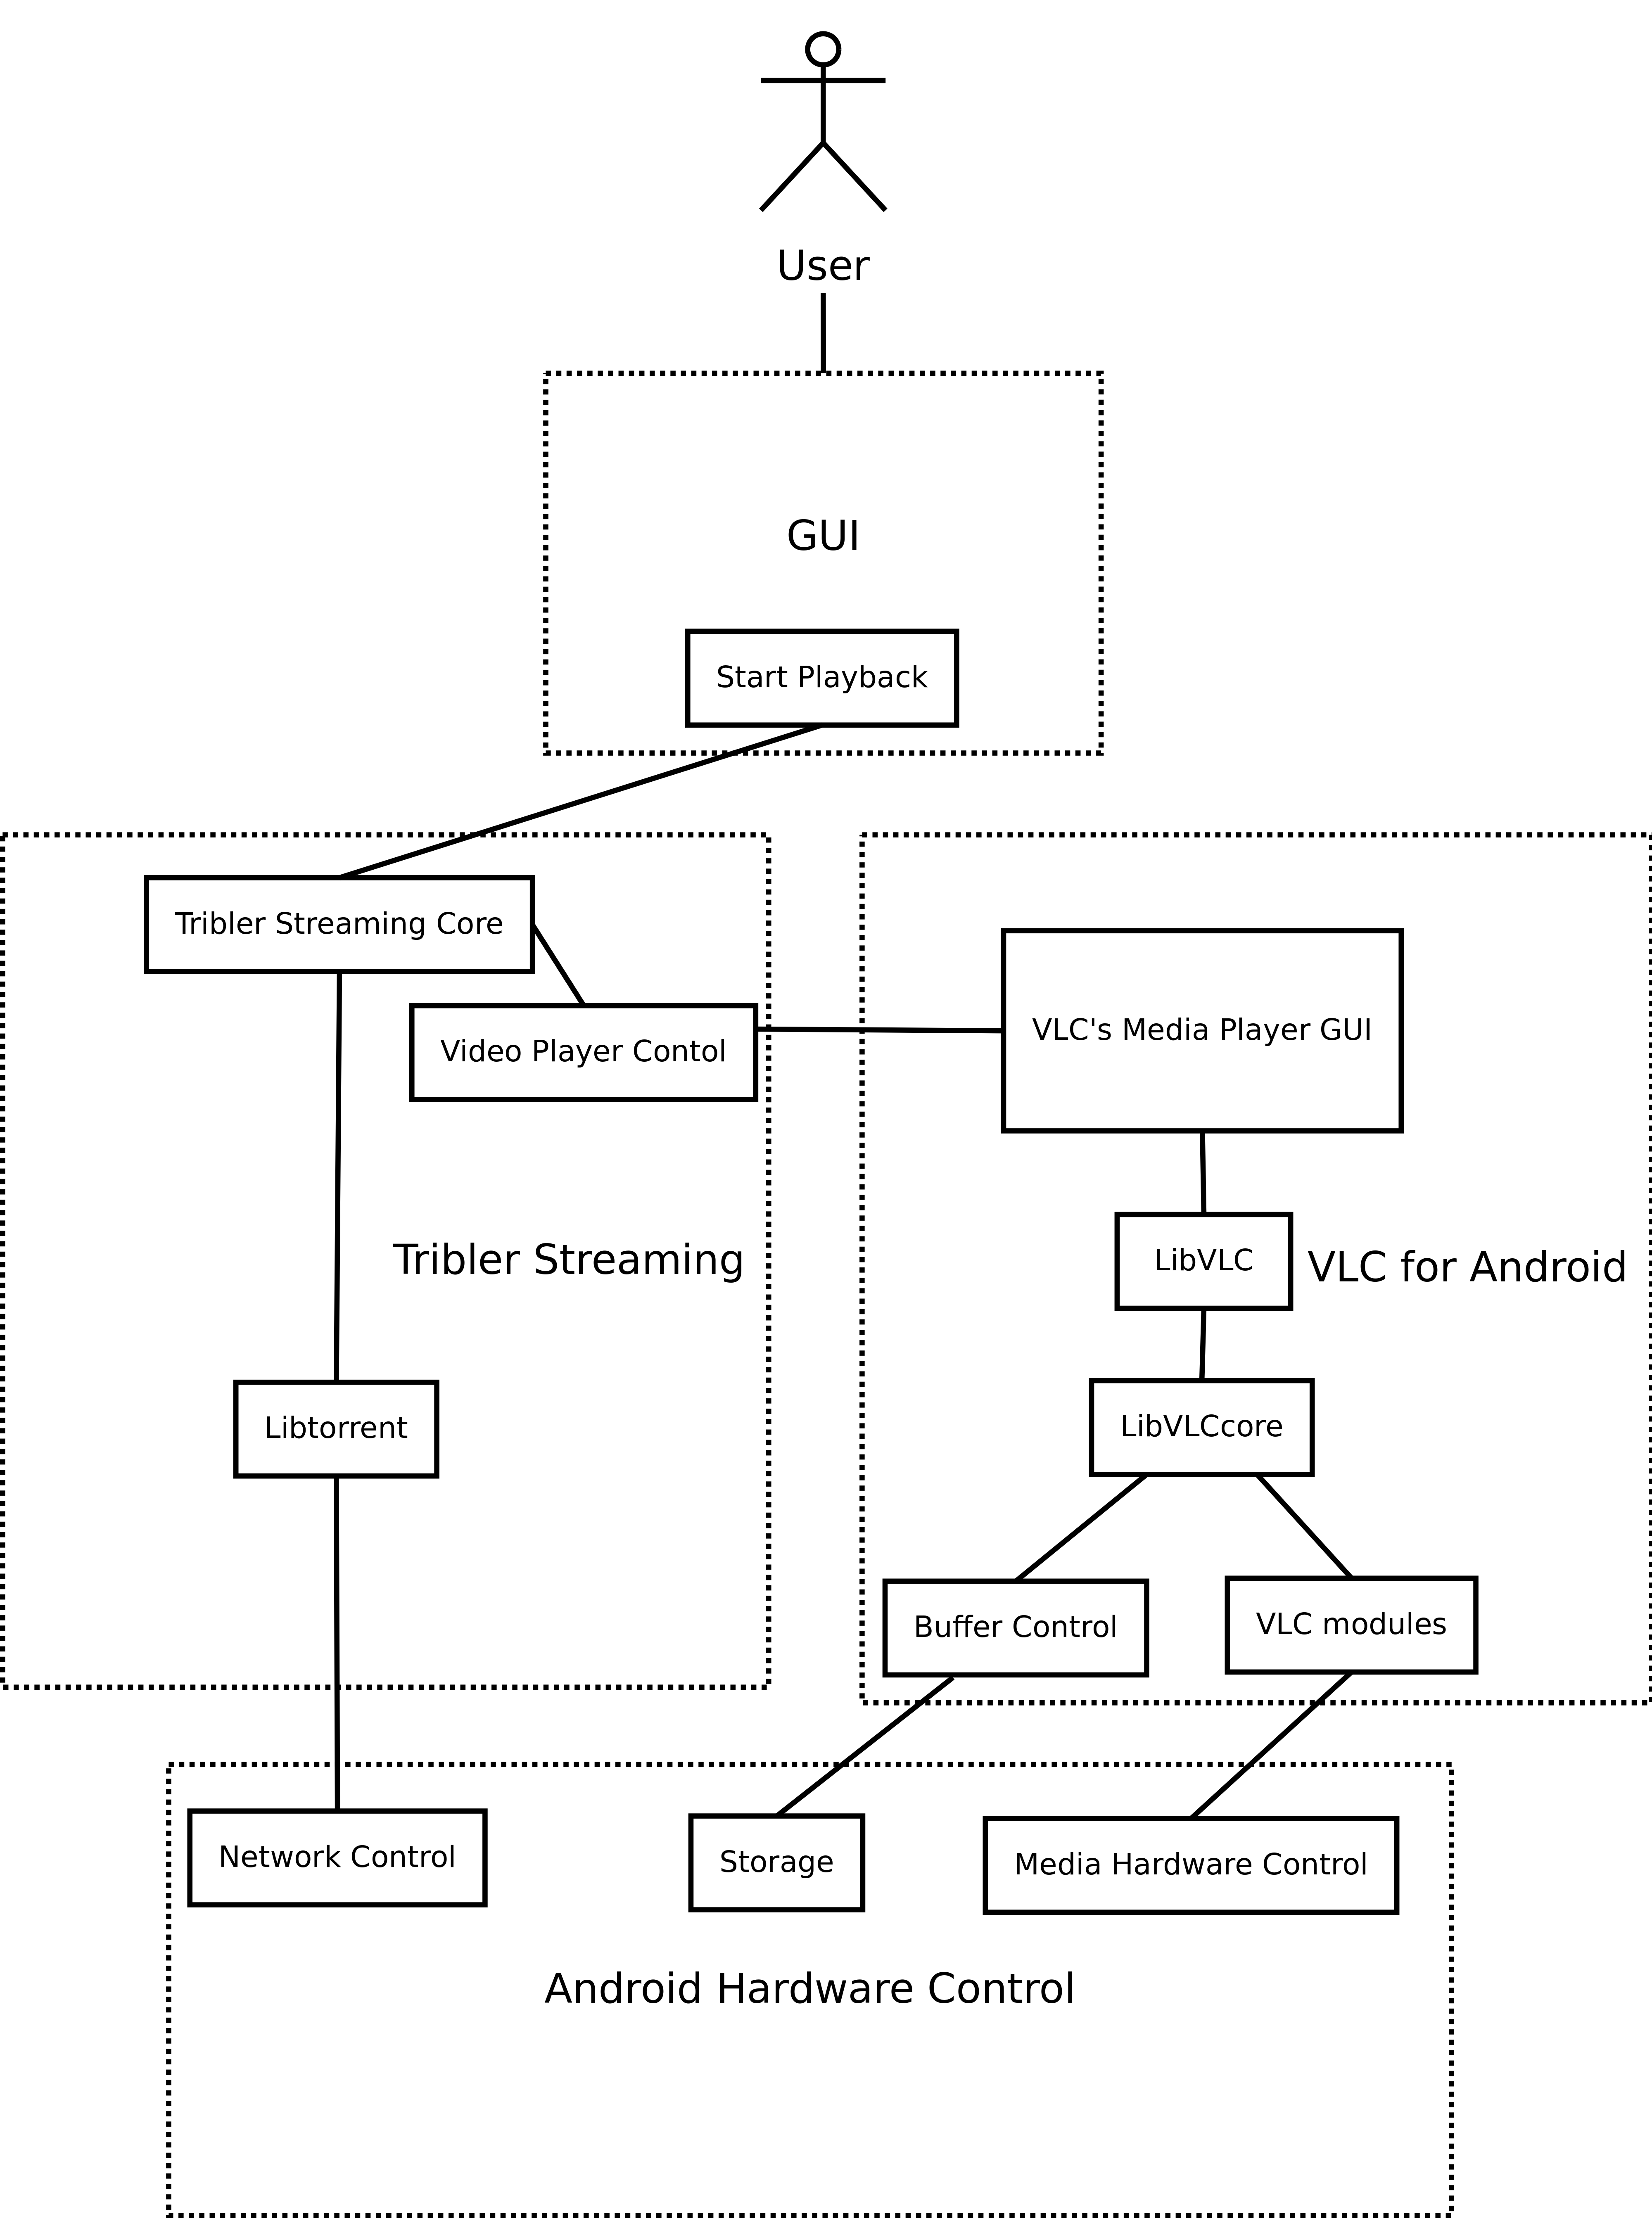
\includegraphics[width=\textwidth]{contents/ad/images/proposed_architecture.png}
	\caption{The proposed architecture of the prototype}
	\label{fig:prop_arch}
\end{figure}
In Figure \ref{fig:prop_arch} a visual overview of the proposed architecture can be found. In this figure, the different subsystem are combined in to one system. At the top sits the user which issues the command to the GUI to start the process of streaming a video. It will then switch to another GUI, which VLC provides, for media playback (VLC's Media Player GUI). The user can play and pause the video as well as seek in the video via this GUI. After the user issues the command to start playback, the Tribler subsystem will download pieces from the video with the Libtorrent protocol. It will store those pieces so that the VLC subsystem can show them to the user when there are enough pieces for continues playback. VLC does this by filling a buffer and letting the player use that for continues playback. The Media Player lets the Video Player Control know what the playback position is so that Libtorrent can download the proper pieces for playback as explained in the subsystems section. The Android Hardware Control subsystem is added to clarify that the interaction with hardware is mostly handled by the Android platform. To clarify, the part that the Team will code themselves, is the Tribler core and the video player control module. The rest may undergo a few minute changes, but will be kept as is to facilitate updates.			%section
\pagebreak
\section{Persistent data management}
\label{sec:perdata}
The prototype application will have to be able to stream high definition videos that in case of Blu-ray video, can have a bitrate of up to 40 Mbit/s.\footnote{http://www.blu-raydisc.com/Assets/Downloadablefile/BD-ROM-AV-WhitePaper_100604\%281\%29-15916-18123.pdf}. In case a video is encoded in DivX Plus HD 1080p format, it can have a maximum bitrate of 20 Mbit/s.\footnote{http://www.divx.com/files/DivX_Plus_HD_Brochure.pdf} In order to decode video streams with such bitrates in real-time, data will have to be downloaded into RAM, after which it can directly decoded. The contiguous pieces that are downloaded from the peers will therefore be stored in a buffer that resides in RAM. At the same time, the piece can also be stored to non-volatile storage such as onboard Flash Memory, or to an external SD-card in case recording of the video stream is required.
		%section
\section{Concurrency}
					%section
\section{Software control}
%how is the control flow within the system				%section
\section{Boundary Conditions}
The prototype application will run on an Android-based mobile device and will communicate with other peers through the Internet using the BitTorrent protocol. Therefore in order for the prototype application to work, an Internet connection is required. The bandwidth of the Internet connection should be equivalent to an average broadband DSL connection (10-20Mbit/s). Once the system is started it can be closed either by selecting `close' from a context menu, by terminating the application with the task manager in Android, or by rebooting the device. In order to facilitate smooth video playback, the device on which the prototype is run should contain hardware that is capable of playing back (decoding) 1080p at 30 fps. 
			%section
\pagebreak
\begin{thebibliography}{9}

\bibitem{libswift12}
   R. Petrocco, J. Pouwelse and D.H.J. Epema,
  \emph{Performance Analysis of the Libswift P2P Streaming Protocol},
  IEEE P2P, TU Delft,
  2012.
\end{thebibliography}
\end{document}
